\documentclass[14pt,a4paper,report]{report}
\usepackage[a4paper, mag=1000, left=2.5cm, right=1cm, top=2cm, bottom=2cm, headsep=0.7cm, footskip=1cm]{geometry}
\usepackage[utf8]{inputenc}
\usepackage[english,russian]{babel}
\usepackage{indentfirst}
\usepackage[dvipsnames]{xcolor}
\usepackage[colorlinks]{hyperref}
\usepackage{listings} 
\usepackage{fancyhdr}
\usepackage{caption}
\usepackage{amsmath}
\usepackage{latexsym}
\usepackage{graphicx}
\usepackage{amsmath}
\usepackage{booktabs}
\usepackage{array}
\hypersetup{
	colorlinks = true,
	linkcolor  = black
}

\usepackage{titlesec}
\titleformat{\chapter}
{\Large\bfseries} % format
{}                % label
{0pt}             % sep
{\huge}           % before-code


\DeclareCaptionFont{white}{\color{white}} 

% Listing description
\usepackage{listings} 
\DeclareCaptionFormat{listing}{\colorbox{gray}{\parbox{\textwidth}{#1#2#3}}}
\captionsetup[lstlisting]{format=listing,labelfont=white,textfont=white}
\lstset{ 
	% Listing settings
	inputencoding = utf8,			
	extendedchars = \true, 
	keepspaces = true, 			  	 % Поддержка кириллицы и пробелов в комментариях
	language = Matlab,            	 	 % Язык программирования (для подсветки)
	basicstyle = \small\sffamily, 	 % Размер и начертание шрифта для подсветки кода
	numbers = left,               	 % Где поставить нумерацию строк (слева\справа)
	numberstyle = \tiny,          	 % Размер шрифта для номеров строк
	stepnumber = 1,               	 % Размер шага между двумя номерами строк
	numbersep = 5pt,              	 % Как далеко отстоят номера строк от подсвечиваемого кода
	backgroundcolor = \color{white}, % Цвет фона подсветки - используем \usepackage{color}
	showspaces = false,           	 % Показывать или нет пробелы специальными отступами
	showstringspaces = false,    	 % Показывать или нет пробелы в строках
	showtabs = false,           	 % Показывать или нет табуляцию в строках
	frame = single,              	 % Рисовать рамку вокруг кода
	tabsize = 2,                  	 % Размер табуляции по умолчанию равен 2 пробелам
	captionpos = t,             	 % Позиция заголовка вверху [t] или внизу [b] 
	breaklines = true,           	 % Автоматически переносить строки (да\нет)
	breakatwhitespace = false,   	 % Переносить строки только если есть пробел
	escapeinside = {\%*}{*)}      	 % Если нужно добавить комментарии в коде
}

\begin{document}

\def\contentsname{Содержание}

% Titlepage
\begin{titlepage}
	\begin{center}
		\textsc{Санкт-Петербургский Политехнический 
			Университет Петра Великого\\[5mm]
			Кафедра компьютерных систем и программных технологий}
		
		\vfill
		
		\textbf{Отчёт по лабораторной работе №2\\[3mm]
			Курс: «Методы оптимизации и принятия решений»\\[3mm]
			Тема: «Анализ GERT-сети»\\[35mm]
			}
	\end{center}
	
	\hfill
	\begin{minipage}{.5\textwidth}
		Выполнил студент:\\[2mm] 
		Ерниязов Тимур Ертлеуевич\\
		Группа: 13541/2\\[5mm]
		
		Проверил:\\[2mm] 
		Сиднев Александр Георгиевич
	\end{minipage}
	\vfill
	\begin{center}
		Санкт-Петербург\\ \the\year\ г.
	\end{center}
\end{titlepage}

% Contents
\tableofcontents
\clearpage

\chapter{Лабораторная работа №2}

\section{Задание}

\begin{figure}[h!]
	\centering
	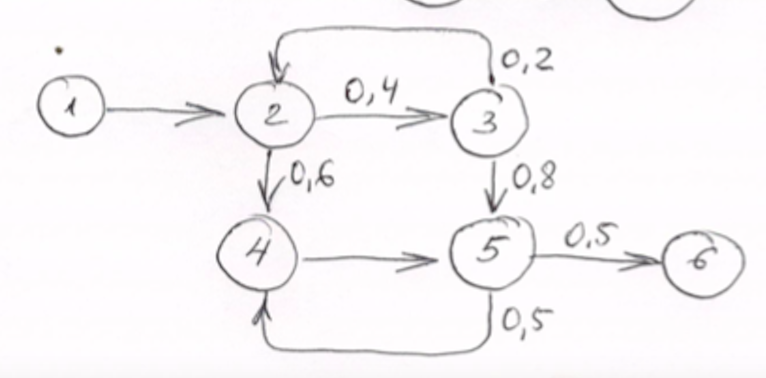
\includegraphics[scale = 0.55]{images/0.png}
	\caption{Исходный граф системы}
	\label{image:0}
\end{figure}

\subsubsection{Часть 1}

Каждой дуге ($ij$) поставлены в соответствие следующие данные:

\begin{itemize}
	\item закон распределения времени выполнения работы (будем считать его нормальным);
	\item параметры закона распределения; (математическое ожидание $M$ и дисперсия $D$).
	\item вероятность $P_{ij}$ выполнения работы, показанная на графе.
\end{itemize}

Необходимо найти:

\begin{itemize}
	\item вероятность выхода в завершающий узел графа (для всех вариантов узел 6);
	\item математическое ожидание;
	\item дисперсию времени выхода процесса в завершающий узел графа;
		\item начальные моменты первых 10 порядков.
\end{itemize}

В отчете перечислить все петли всех порядков, обнаруженные на графе, выписать уравнение Мейсона, получить решение для $W_E(s)$ и найти требуемые параметры.

\subsubsection{Часть 2}

Решить задачу используя методику анализа потокового графа, основанную на обработке матрицы передач (Branch Transmittance Matrix).

\clearpage

\section{Ход работы}

\subsection{Построение замкнутой GERT-сети}

Чтобы определить эквивалентную W-функцию для анализируемой GERT-сети, необходимо замкнуть сеть дугой, исходящей из узла 6 в узел 1:

\begin{figure}[h!]
	\centering
	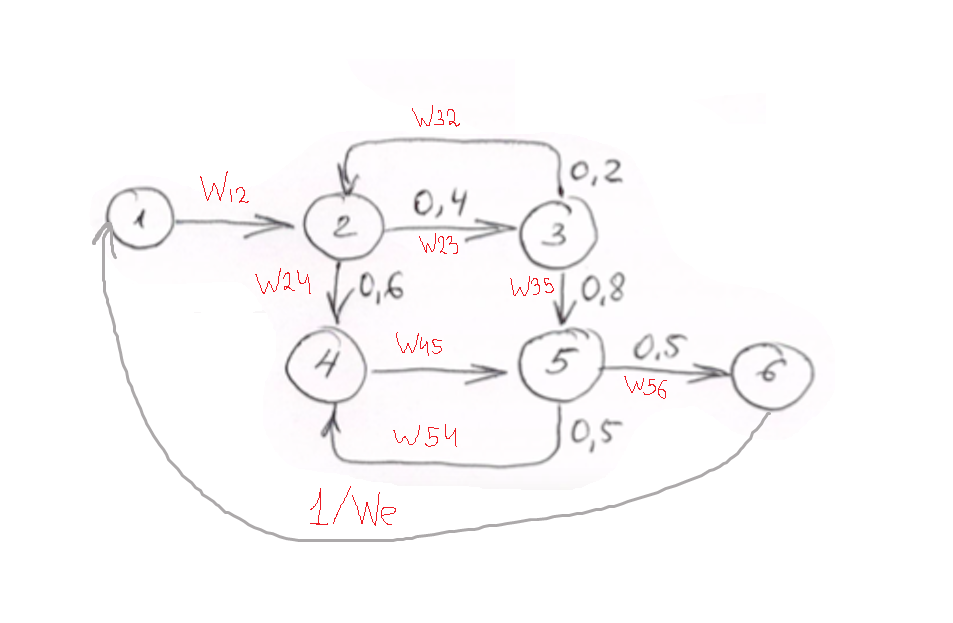
\includegraphics[scale = 0.65]{images/1.png}
	\caption{Замкнутая GERT-сеть}
	\label{image:1}
\end{figure}

\subsection{Построение W-функции}

Найдем W-функции для дуг GERT-сети:

\begin{table}[h!]
	\bgroup
	\def\arraystretch{1}
	\begin{tabular}{ | m{1.5cm} | m{1.5cm} | m{2.0cm} | m{1.0cm} | m{1.0cm} | m{5.0cm} | }
		\hline
		Начало & Конец & Вероятность & M & D & W-функция \\ \hline
		1 &  2 & 1 		& 44 & 25 & $(0.0014348 (e^{8.8 s} - 1 e^{35.2 s})^2)/s^2$ \\ \hline
		2 & 3 & 0.4  & 24 & 25 & $(0.00192901 (e^{4.8 s} - 1 e^{19.2 s})^2)/s^2$ \\ \hline
		2 & 4 & 0.6 	& 40 & 25 & $(0.00104167 (e^{8 s} - 1 e^{32 s})^2)/s^2$ \\ \hline
		3 & 2 & 0.2 	& 34 & 25 & $(0.00048058 (e^{6.8 s} - 1 e^{27.2 s})^2)/s^2$ \\ \hline
		3 & 5 & 0.8 	& 15 & 9 &    $(0.00987654 (e^{3 s} - 1 e^{12 s})^2)/s^2$ \\ \hline
		4 & 5 & 1 		& 32 & 25 & $(0.00271267 (e^{6.4 s} - 1 e^{25.6 s})^2)/s^2$ \\ \hline
		5 & 4 & 0.5 	& 11 & 4 &    $(0.0114784 (e^{2.2 s} - 1 e^{8.8 s})^2)/s^2$ \\ \hline
		5 & 6 & 0.5 	& 24 & 25 & $(0.00241127 (e^{4.8 s} - 1 e^{19.2 s})^2)/s^2$ \\ \hline
	\end{tabular}
	\egroup
\end{table}

\subsection{Построение уравнения Мейсона}

Петли первого порядка:

$W_{45}\cdot W_{54}$

$W_{23}\cdot W_{32}$

$W_{12}\cdot W_{23}\cdot W_{35}\cdot W_{56}\frac{1}{W_E}$

$W_{12}\cdot W_{24}\cdot W_{45}\cdot W_{56}\frac{1}{W_E}$

Петли второго порядка:
$W_{23}\cdot W_{32}\cdot W_{45}\cdot W_{54}$

Таким образом уравнение Мейсона будет иметь следующий вид:

$H=1 - W_{45}W_{54}
-W_{23}W_{32}
-W_{12}W_{23}W_{35}W_{56}\frac{1}{W_E}
-W_{12}W_{24}W_{45}W_{56}\frac{1}{W_E}
+W_{23}W_{32}W_{45}W_{54}$\\

В результате эквивалентная W-функция равняется:

$W_E(s)=- \frac{W_{12}W_{23}W_{35}W_{56}+
-W_{12}W_{24}W_{45}W_{56}}
{W_{23}W_{32}
+W_{45}W_{54}
+W_{23}W_{32}W_{45}W_{54}
-1}$\\

\subsection{Рассчет статистических значений}

Расчет математического ожидания ($\mu_{1E}$) и дисперсии ($\sigma_E$) производится по следующим образом:

$$\mu_{1E}=\frac{d M_E(s)}{ds}|s=0$$

$$\mu_{2E}=\frac{d^2 M_E(s)}{ds^2}|s=0$$

$$\sigma^2=\mu_{2E}-\mu_{1E}^2$$

$$ p_E=W_E(0)$$

Разработаем скрипт для расчета статистических значений в среде MATLAB:
\begin{lstlisting}[language={matlab}, caption={Matlab скрипт}, basicstyle=\ttfamily]
P12 = 1;   M12 = 44; D12 = 25;
P23 = 0.4; M23 = 24; D23 = 25;
P24 = 0.6;   M24 = 40; D24 = 25;
P32 = 0.2; M32 = 34; D32 = 25;
P35 = 0.8;   M35 = 15; D35 = 9;
P45 = 1; M45 = 32; D45 = 25;
P54 = 0.5; M54 = 11; D54 = 4;
P56 = 0.5; M56 = 24; D56 = 25;

syms s

W12 = P12*((2*(exp((s*1.6*M12)/2)-exp((s*0.4*M12)/2)))/((1.6*M12-0.4*M12)*s))^2;
W23 = P23*((2*(exp((s*1.6*M23)/2)-exp((s*0.4*M23)/2)))/((1.6*M23-0.4*M23)*s))^2;
W24 = P24*((2*(exp((s*1.6*M24)/2)-exp((s*0.4*M24)/2)))/((1.6*M24-0.4*M24)*s))^2;
W35 = P35*((2*(exp((s*1.6*M35)/2)-exp((s*0.4*M35)/2)))/((1.6*M35-0.4*M35)*s))^2;
W45 = P45*((2*(exp((s*1.6*M45)/2)-exp((s*0.4*M45)/2)))/((1.6*M45-0.4*M45)*s))^2;
W32 = P32*((2*(exp((s*1.6*M32)/2)-exp((s*0.4*M32)/2)))/((1.6*M32-0.4*M32)*s))^2;
W54 = P54*((2*(exp((s*1.6*M54)/2)-exp((s*0.4*M54)/2)))/((1.6*M54-0.4*M54)*s))^2;
W56 = P56*((2*(exp((s*1.6*M56)/2)-exp((s*0.4*M56)/2)))/((1.6*M56-0.4*M56)*s))^2;

We = ((W12*W23*W35*W56+W12*W24*W45*W56)/(1-W45*W54-W23*W32+W23*W32*W45*W54));
We = simplify(We);

We0 = limit(We, 's', 0)

Me = We / We0;

me1 = diff(Me, 's', 1);
me1 = limit(me1, 's', 0)
me2 = diff(Me, 's', 2);
me2 = limit(me2, 's', 0)

de = me2 - me1 ^ 2
\end{lstlisting}


Результат вычисления статистических значений:

\begin{lstlisting}[language={matlab}, caption={Matlab скрипт}, basicstyle=\ttfamily]
We0 =1
 
me1 =4061/23 
 
me2 =946542817/26450 
 
de =121956767/26450
\end{lstlisting}

Были получены следующие результаты:
\begin{enumerate}
\item Вероятность выхода в завершающий узел графа равна 100\% ($p=W_E=1$).
\item Математическое ожидание 4061/23 (176.57).
\item Дисперсия времени выхода процесса в завершающий узел графа 121956767/26450 (4 610,84).
\end{enumerate}

\subsection{Часть 2}

Определим матрицу Q:
\begin{equation*}
Q = 
 \begin{pmatrix}
  0 & q_{12} & 0 & 0 & 0 & 0 \\
  0 & 0 & q_{23} & q_{24} & 0 & 0 \\ 
  0 & q_{32} & 0 & 0 & q_{35} & 0 \\ 
  0 & 0 & 0 & 0 & q_{45} & 0 \\ 
  0 & 0 & 0 & q_{54} & 0 & q_{56} \\ 
  w_{61} & 0 & 0 & 0 & 0 & 0 
 \end{pmatrix}
\end{equation*}
Определим матрицу коэффициентов $A=I_6-Q^T$.
\begin{equation*}
A = 
 \begin{pmatrix}
    1&       0&    -q_{31}&    0&    0& -w_{61}\\
 -q_{12} & 1 & 0&    0&       0&    0\\
    0&    -q_{23}&    1&    0&       -q_{53}&    0\\
    0&       -q_{24}& -q_{34}&    1&       0&    0\\
    0&       0&    0& -q_{45}& 1 &    0\\
    0&       0&    0&    -q_{46}&    -q_{56}&    1
 \end{pmatrix}
\end{equation*}
Находим 
\begin{equation*}
det(A)
\end{equation*}
далее
\begin{equation*}
\frac{\partial det(A)}{\partial w_{61}}
\end{equation*}
\begin{equation*}
det(A | w_{61}=0)
\end{equation*}
Далее можно вывести $W_E(S)$ с помощью формулы:
\begin{equation*}
W_E(S)=-\frac{\frac{\partial det(A)}{\partial w_{61}}}{det(A | w_{61}=0)}
\end{equation*}
Для расчетов, был написан matlab скрипт.
\begin{lstlisting}[language={matlab}, caption={Matlab скрипт}, basicstyle=\ttfamily]
P12 = 1;   M12 = 44; 
P23 = 0.4; M23 = 24; 
P24 = 0.6;   M24 = 40; 
P32 = 0.2; M32 = 34; 
P35 = 0.8;   M35 = 15; 
P45 = 1; M45 = 32; 
P54 = 0.5; M54 = 11; 
P56 = 0.5; M56 = 24;

syms q12
syms q23
syms q24
syms q32
syms q35
syms q45
syms q54
syms q56
syms w61
syms s

Q=[0 q12 0 0 0 0;
   0 0 q23 q24 0 0;
   0 q32 0 0 q35 0;
   0 0 0 0 q45 0;
   0 0 0 q54 0 q56;
   w61 0 0 0 0 0];

A1 = eye(size(Q,1)) - transpose(Q);
det_A1 = det(A1);
det_dw=diff(det_A1, w61);
det2_A1=subs(det_A1, w61, 0);
We = -det_dw/det2_A1

We=subs(We, q12, P12*((2*(exp((s*1.6*M12)/2)-exp((s*0.4*M12)/2)))/((1.6*M12-0.4*M12)*s))^2);
We=subs(We, q23, P23*((2*(exp((s*1.6*M23)/2)-exp((s*0.4*M23)/2)))/((1.6*M23-0.4*M23)*s))^2);
We=subs(We, q24, P24*((2*(exp((s*1.6*M24)/2)-exp((s*0.4*M24)/2)))/((1.6*M24-0.4*M24)*s))^2);
We=subs(We, q32, P32*((2*(exp((s*1.6*M32)/2)-exp((s*0.4*M32)/2)))/((1.6*M32-0.4*M32)*s))^2);
We=subs(We, q45, P45*((2*(exp((s*1.6*M45)/2)-exp((s*0.4*M45)/2)))/((1.6*M45-0.4*M45)*s))^2);
We=subs(We, q54, P54*((2*(exp((s*1.6*M54)/2)-exp((s*0.4*M54)/2)))/((1.6*M54-0.4*M54)*s))^2);
We=subs(We, q56, P56*((2*(exp((s*1.6*M56)/2)-exp((s*0.4*M56)/2)))/((1.6*M56-0.4*M56)*s))^2);
We=subs(We, q35, P35*((2*(exp((s*1.6*M35)/2)-exp((s*0.4*M35)/2)))/((1.6*M35-0.4*M35)*s))^2);

We = simplify(We);
We0 = limit(We, 's', 0)
Me = We / We0;

me1 = diff(Me, 's', 1);
me1 = limit(me1, 's', 0)
me2 = diff(Me, 's', 2);
me2 = limit(me2, 's', 0)

de = me2 - me1 ^ 2
\end{lstlisting}

\begin{lstlisting}[language={matlab}, caption={Результат}, basicstyle=\ttfamily]
We = -(q12*q23*q35*q56 + q12*q24*q45*q56)/(q23*q32 + q45*q54 - q23*q32*q45*q54 - 1)
 
We0 =1
 
me1 =4061/23
 
me2 =946542817/26450
 
de =121956767/26450
\end{lstlisting}

Были получены следующие результаты:
\begin{enumerate}
\item Вероятность выхода в завершающий узел графа равна 100\% ($p=W_E=1$).
\item Математическое ожидание 4061/23 (176.57).
\item Дисперсия времени выхода процесса в завершающий узел графа 121956767/26450 (4 610,84).
\end{enumerate}
Которые полностью совпадает с результатами части 1.



\section{Вывод}

В ходе данной лабораторной работы были получены навыки работы с вероятностными графами и их обработка с помощью методики GERT. При заданных значениях вероятности, мат. ожидания для каждой дуги исходного графа достаточно легко расчитываются W-функции для треугольного распределения, которые необходимы для построения формулы Мейсона. После этого из формулы Мейсона по формулам математической статистики достаточно легко расчитывается результирующее мат. ожидание и дисперсия.

Решение путем анализа потокового графа показало аналогичные результаты, что подтверждает корректность решения. Однако, метод анализа потокового графа выполняется заметно медленнее, даже на небольшом графе.

\end{document}